% Figure F2_heldout_over_iterations of study_analysis_001 - generated by thesis/study_analysis/figures.py; do not edit by hand.
% Preamble: \usepackage{pgfplots}
%           \pgfplotsset{compat=1.18}
% ParEval vs held-out pass rate over repair steps
% Caption: figures/F2_heldout_over_iterations.caption.tex (figure_caption_tex)
% Composite block; Q06 correctness pass (solid) and E02 enhanced all-pass (dashed) on the identical base-cell cohort per step (G02 overfitting check); STEP[v][0] == BASE and STEP[v][2] == FINAL[v] (checked)
% y axis truncated: it starts at 80%, not at 0 (data-driven lower bound floor((min - 2) / 5) * 5 over the plotted values and CI bounds); the series are dodged horizontally by 0.04 steps so that the error bars do not overlap
% error bars: 95% CI: nonparametric cluster bootstrap, percentile intervals, stratified by block (pilot benchmarks resampled among the 12 pilot benchmarks, full_ext among its 48); seed 20261017; cluster = benchmark; 2,000 replicates (descriptive, unadjusted)
% BL01: Includes dense_la/00 (BL-01 tolerance convention: possible false FAIL verdicts; disclosure-bearing aggregate); sensitivity SA1 in T10.
% IC1: Q06 is in-sample for test_feedback and combined_feedback: their loops see the ParEval test verdict and stop when it passes (every stopped_tests_pass trajectory is a Q06 pass), so they optimise the endpoint; for static_feedback Q06 is out-of-sample (measured once in phase 2, never seen by the loop). The variants therefore differ in trigger and stop rules, not only in feedback content; test_feedback cannot regress on Q06 by construction.
% IC2: E02 is not an independent confirmation of Q06 gains: it counts build failures, and most E02 improvements are the same cells as the Q06 improvements; the held-out signal proper is the joint transition X06 (e.g. Q06 repaired but E02 still failing) and G01.
% IC6: static_feedback repair triggers are dominated by clang-tidy bugprone findings and, on MPI, by low-confidence hints (design document: no trustworthy static MPI tool exists); static_feedback results measure this frozen blocking-set configuration, not static analysis in general.
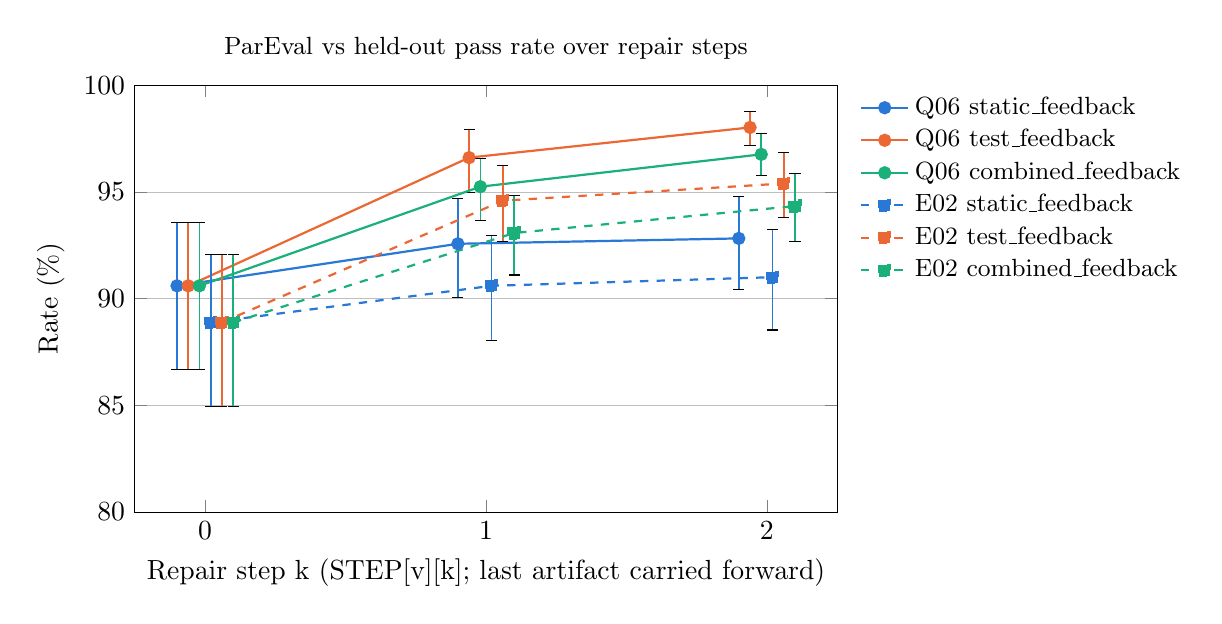
\begin{tikzpicture}
\definecolor{saSeriesA}{HTML}{2A78D6}
\definecolor{saSeriesB}{HTML}{EB6834}
\definecolor{saSeriesC}{HTML}{1BAF7A}
\definecolor{saSeriesD}{HTML}{2A78D6}
\definecolor{saSeriesE}{HTML}{EB6834}
\definecolor{saSeriesF}{HTML}{1BAF7A}
\begin{axis}[
  width=10.5cm,
  height=7cm,
  xmin=-0.250,
  xmax=2.250,
  xtick={0,1,2},
  ymin=80.000,
  ymax=100.000,
  xlabel={Repair step k (STEP[v][k]; last artifact carried forward)},
  ylabel={Rate (\%)},
  ymajorgrids,
  legend cell align=left,
  legend style={at={(1.02,1)},anchor=north west,font=\small,draw=none},
  title={ParEval vs held-out pass rate over repair steps},
  title style={font=\small}
]
\addplot[color=saSeriesA, thick, mark=*, solid] coordinates {(-0.100,90.606) (0.900,92.576) (1.900,92.828)};
\addlegendentry{Q06 static\_feedback}
\addplot[forget plot, draw=none, mark=none, error bars/.cd, y dir=both, y explicit, error bar style={draw=saSeriesA, solid, line width=0.6pt}] coordinates {(-0.100,90.606) += (0,2.981) -= (0,3.941) (0.900,92.576) += (0,2.121) -= (0,2.525) (1.900,92.828) += (0,1.970) -= (0,2.374)};
\addplot[color=saSeriesB, thick, mark=*, solid] coordinates {(-0.060,90.606) (0.940,96.616) (1.940,98.030)};
\addlegendentry{Q06 test\_feedback}
\addplot[forget plot, draw=none, mark=none, error bars/.cd, y dir=both, y explicit, error bar style={draw=saSeriesB, solid, line width=0.6pt}] coordinates {(-0.060,90.606) += (0,2.981) -= (0,3.941) (0.940,96.616) += (0,1.313) -= (0,1.617) (1.940,98.030) += (0,0.758) -= (0,0.859)};
\addplot[color=saSeriesC, thick, mark=*, solid] coordinates {(-0.020,90.606) (0.980,95.253) (1.980,96.768)};
\addlegendentry{Q06 combined\_feedback}
\addplot[forget plot, draw=none, mark=none, error bars/.cd, y dir=both, y explicit, error bar style={draw=saSeriesC, solid, line width=0.6pt}] coordinates {(-0.020,90.606) += (0,2.981) -= (0,3.941) (0.980,95.253) += (0,1.313) -= (0,1.567) (1.980,96.768) += (0,0.960) -= (0,1.010)};
\addplot[color=saSeriesD, thick, mark=square*, dashed] coordinates {(0.020,88.889) (1.020,90.606) (2.020,91.010)};
\addlegendentry{E02 static\_feedback}
\addplot[forget plot, draw=none, mark=none, error bars/.cd, y dir=both, y explicit, error bar style={draw=saSeriesD, solid, line width=0.6pt}] coordinates {(0.020,88.889) += (0,3.182) -= (0,3.939) (1.020,90.606) += (0,2.374) -= (0,2.576) (2.020,91.010) += (0,2.222) -= (0,2.475)};
\addplot[color=saSeriesE, thick, mark=square*, dashed] coordinates {(0.060,88.889) (1.060,94.596) (2.060,95.404)};
\addlegendentry{E02 test\_feedback}
\addplot[forget plot, draw=none, mark=none, error bars/.cd, y dir=both, y explicit, error bar style={draw=saSeriesE, solid, line width=0.6pt}] coordinates {(0.060,88.889) += (0,3.182) -= (0,3.939) (1.060,94.596) += (0,1.667) -= (0,1.919) (2.060,95.404) += (0,1.465) -= (0,1.616)};
\addplot[color=saSeriesF, thick, mark=square*, dashed] coordinates {(0.100,88.889) (1.100,93.081) (2.100,94.343)};
\addlegendentry{E02 combined\_feedback}
\addplot[forget plot, draw=none, mark=none, error bars/.cd, y dir=both, y explicit, error bar style={draw=saSeriesF, solid, line width=0.6pt}] coordinates {(0.100,88.889) += (0,3.182) -= (0,3.939) (1.100,93.081) += (0,1.768) -= (0,1.970) (2.100,94.343) += (0,1.515) -= (0,1.667)};
\end{axis}
\end{tikzpicture}
